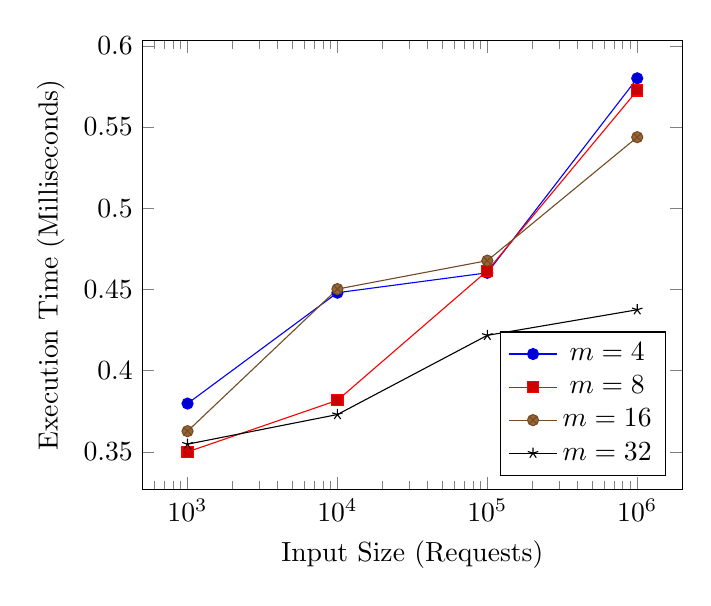
\begin{tikzpicture}
	\begin{axis}
		[
			xlabel={Input Size (Requests)},
			ylabel={Execution Time (Milliseconds)},
			legend pos=south east,
			domain=1:1000000,
			xmode=log,
		]
		\addplot+[cycle list name=color list]
			coordinates {
				(1000, 0.37975)
				(10000, 0.448)
				(100000, 0.46025)
				(1000000, 0.58)
			};
		\addlegendentry{$m=4$}
		\addplot+[cycle list name=color list]
			coordinates {
				(1000, 0.35)
				(10000, 0.38175)
				(100000, 0.4615)
				(1000000, 0.5725)
			};
		\addlegendentry{$m=8$}
		\addplot+[cycle list name=color list]
			coordinates {
				(1000, 0.36275)
				(10000, 0.45025)
				(100000, 0.46775)
				(1000000, 0.54375)
			};
		\addlegendentry{$m=16$}
		\addplot+[cycle list name=color list]
			coordinates {
				(1000, 0.35475)
				(10000, 0.373)
				(100000, 0.42175)
				(1000000, 0.4375)
			};
		\addlegendentry{$m=32$}
	\end{axis}
\end{tikzpicture}
